\chapter{Geophysics Interferometer (GIF)}



\section{Introduction}
地物干渉計の目的は、地球物理学の現象を精密に測定することと、KAGRAの基線長をモニターすることである。
\subsection{Laser Strainmeter for Geophysics}



\subsection{Motivation in GW detectors}


\section{Working Principle}

\subsection{Asynmetric Michelson Interferometer}

\begin{eqnarray} \label{eq:eq401}
  \phi = 2\pi\frac{2(l_x-l_y)}{\lambda}\sim4\pi\frac{l_x}{\lambda}
\end{eqnarray}

\begin{eqnarray}\label{eq:eq402}
  |d\phi| = 4\pi\frac{l_x}{\lambda}\left( \left|\frac{d\lambda}{\lambda}\right| + \left|\frac{dl_x}{l_x}\right| \right)
\end{eqnarray}


\subsection{Seismic Strain Response}
In order to calculate the response from the seismic strain to the optical phase of the GIF interferometer, the same as the Fig.(\ref{img:img310}), it is assumed that the plane seismic waves which displacement $u(t,x)$ is represented as $u(t,x)=u_0e^{i(\omega{t}-kx)}$ with angular frequency of $\omega$ and wave number of $k$, which propagates along with the direction of the baseline of the strainmeter (right direction in this figure). First, because the length fluctuation between two mirrors sparated with $L$ can be expressed as 
\begin{eqnarray} 
  \Delta{L(t)} &\equiv& u(t,0) - u(t,L) \\
  &=& u(t,0) - u(t-\tau,0), \label{eq:eq403}
\end{eqnarray}
where $\tau=L/v$ is the time delay, the transfer function from the displacement to the length fluctuation is given by Laplace transform as
\begin{eqnarray} \label{eq:eq404}
  H_{\mathrm{disp}}(s) \equiv \frac{\Delta{L(s)}}{u(s)} = \frac{u(s)\left[ 1-\exp(-\tau{s}) \right]}{u(s)} = 1 - \exp(-\tau{s})
\end{eqnarray}
Moreover, because the strain amplitude $\epsilon{(x,t)}$ is defined as $\epsilon{(x,t)}\equiv\frac{du}{dx}$, the seismic strain is represented as 
\begin{eqnarray} 
  \epsilon{(x,t)} \equiv \frac{du}{dx} = \frac{du}{dt} \frac{dt}{dx} =  \frac{du}{dt} \frac{1}{v} \label{eq:eq406}
\end{eqnarray}
Therefore, similarly, the transfer function from the seismic strain to the displacement is given  as
\begin{eqnarray} \label{eq:eq407}
  u(s) = \frac{v}{s} \epsilon(s).
\end{eqnarray}
Finary, because the transfer function from the length change of the baseline to the optical phase is given as $4\pi/{\lambda_{\mathrm{opt}}}$ according to the optical gain in Eq.(\ref{eq:eq401}), the transfer function from the seismic strain to the optical phase is represented as 
\begin{eqnarray} \label{eq:eq407}
  H_{\mathrm{strain}}(s) = 4\pi\frac{1}{\lambda_{\mathrm{opt}}} \left[1 - \exp(-\tau{s}) \right]\frac{v}{s}.
\end{eqnarray}

\begin{figure}[h]
  \centering
  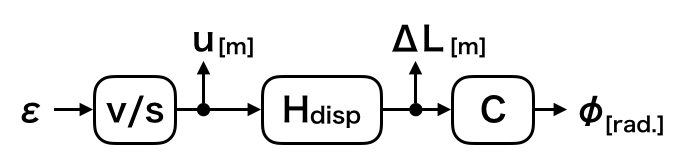
\includegraphics[width=10.0cm]{./img_chap4/img411.png}
  \caption{The response from seismic strain to optical phase. $\epsilon$ is the seismic strain, $u$ is the displacement, $\Delta{L}$ is the length change of the X-arm baseline, and $\phi$ is the optical phase of the GIF interferometer. $C$ is the optical gain of the GIF interferometer given in Eq.(\ref{eq:eq401}). $H_{\mathrm{disp}}$ is the transfer function from the displacement to the length change given in Eq.(\ref{eq:eq404}). $v/s$ is the transfer function from the seismic strain to the displacement given in Eq.(\ref{eq:eq406}). } \label{img:img411}
\end{figure}

As a summary of these transfer function, these are related with each other as shown in Fig.(\ref{img:img411}). Furthermore, we should note the seismic strain reponse depending with the baseline length.

\begin{figure}[p]
  \begin{center}
    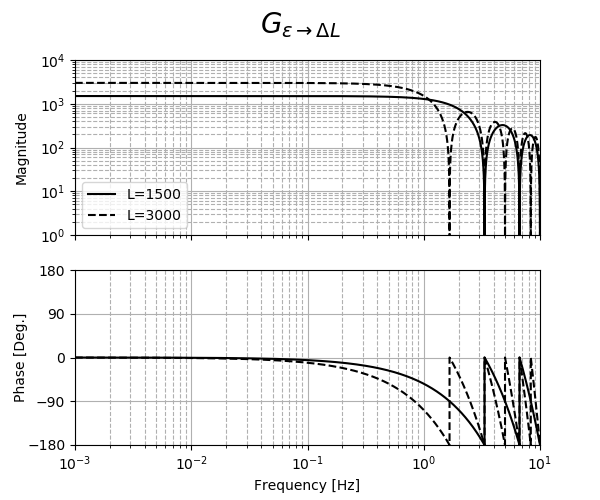
\includegraphics[width=12.0cm]{./img_chap4/img412.png}
    \caption{Compasison of the transfer function from strain of the baseline $\epsilon$ to the length change of that $\Delta{L}$ in the different baseline length. $3000\,\mathrm{m}$ の基線長ではその半分の$1500\,\mathrm{Hz}$よりも、DCゲインは二倍大きい一方で、コーナー周波数は \color{red}{A} になり帯域が減る。また、周波数が \color{red}{B} の条件を満たすとき、ゲインはゼロになる。なぜならば、このときひずみは基線を同相で動かし、基線長伸縮として現れないためである。}
  \end{center}
\end{figure}



\subsection{Quadrature Phase Fringe Detection}
\begin{figure}[h]
  \begin{center}
    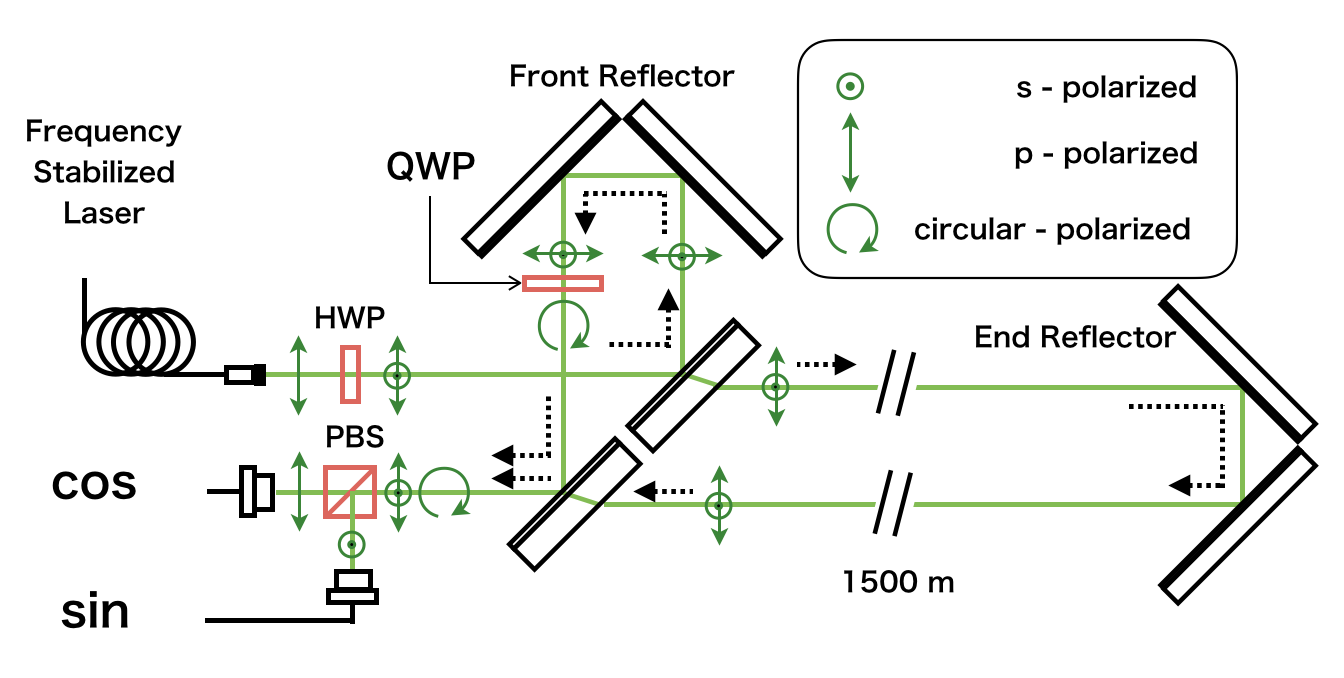
\includegraphics[width=11.0cm]{./img_chap4/img413.png}
    \caption{Quadrature interferometer used in the GIF strainmeter. A half-wave plate (HWP) produces a p-polarization and s-polarization. A quator-wave plate (QWP) delay the optical phase of the s-polarized light with 90 degree against to the another. As a result, one can obtain the quadrature phase fringe.}\label{img:img413}
  \end{center}
\end{figure}

We use the quadrature phase fringe detection to measure the length change of the baseline with wide dynamic range \cite{bobroff1993recent}. The optical layout for the detection is shown in Fig.(\ref{img:img413}). The quadrature phase fringes are detected by two photo detectors, these can be represented as
\begin{eqnarray}
  x &=& x_0 + a \sin(p+p_0), \\
  y &=& y_0 + a \sin(p),
\end{eqnarray}
where $x$ and $y$ are the two voltage outputs from the detectors, $a$ and $b$ are the amplitudes of these fringe signals, $x_0$ and $y_0$ are the offsets, and $p_0$ is the oase offsets from imperfections \cite{zumberge2004resolving}.



\subsection{Noise}


どういうノイズが原理的に存在するか述べる。空気ゆらぎ、周波数雑音を述べる。


\section{Optics Design} %光学系
...\\
\subsection{Overview}
Optical layout is shown in Fig. \ref{img:img}. Optics of GIF is categorized by three category; mode-matching optics, core optics and frequency stabilized laser.

\begin{figure}[h]
  \begin{center}   
    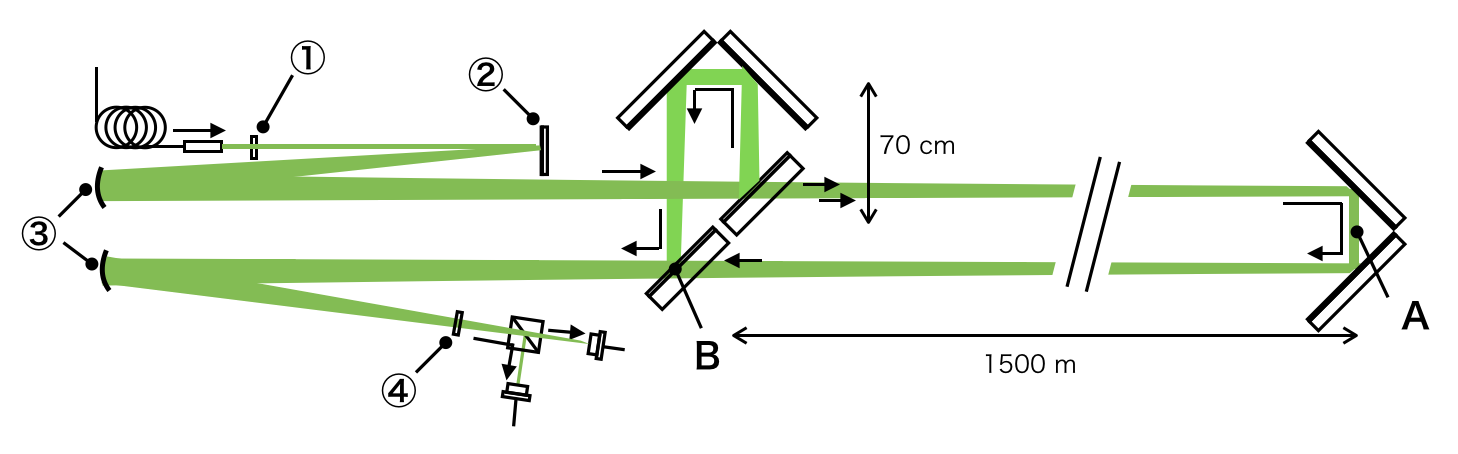
\includegraphics[width=11cm]{./img_chap4/img416.png}
    \caption{Schematic optics layout.}\label{img:img416}
  \end{center}
\end{figure}

\subsection{Input Output Optics}
エンドリフレクタでビームウエストになるようにモードマッチさせている。

\subsection{Core Optics}
The core optics of the Michelson interferometer are composed of two reflectors and beam splitter (BS). 

\begin{figure}[p]  
    \begin{center}   
      %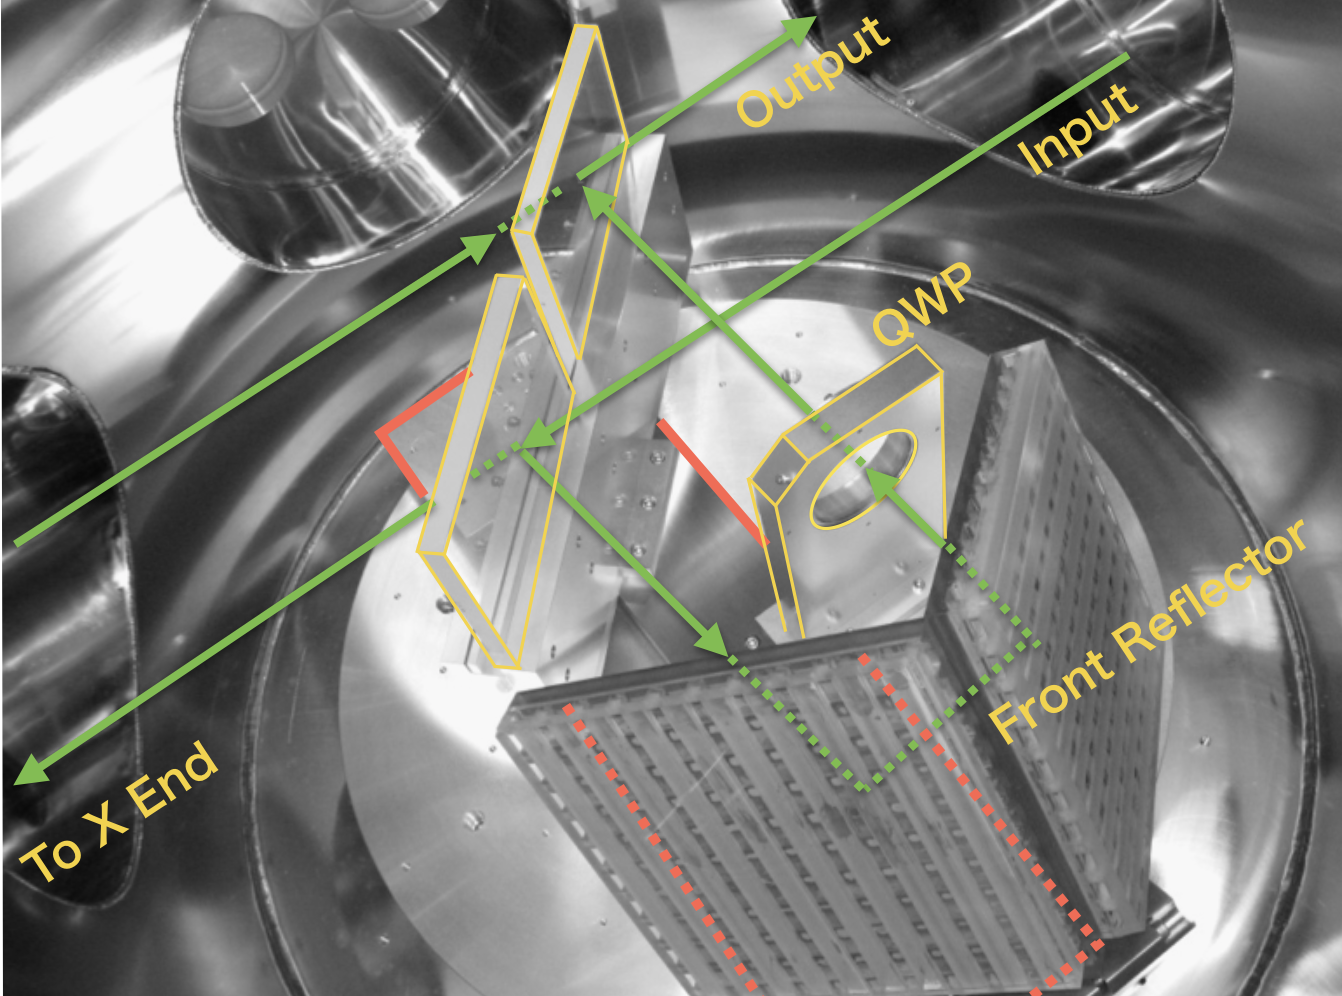
\includegraphics[width=11cm]{./img_chap4/img418.png} % ファイル重い
      
\includegraphics[width=11cm]{./img.png}
      \subcaption{Core optics in the front vacuum chamber. }\label{img:img418}
    \end{center}
    \begin{center}   
      %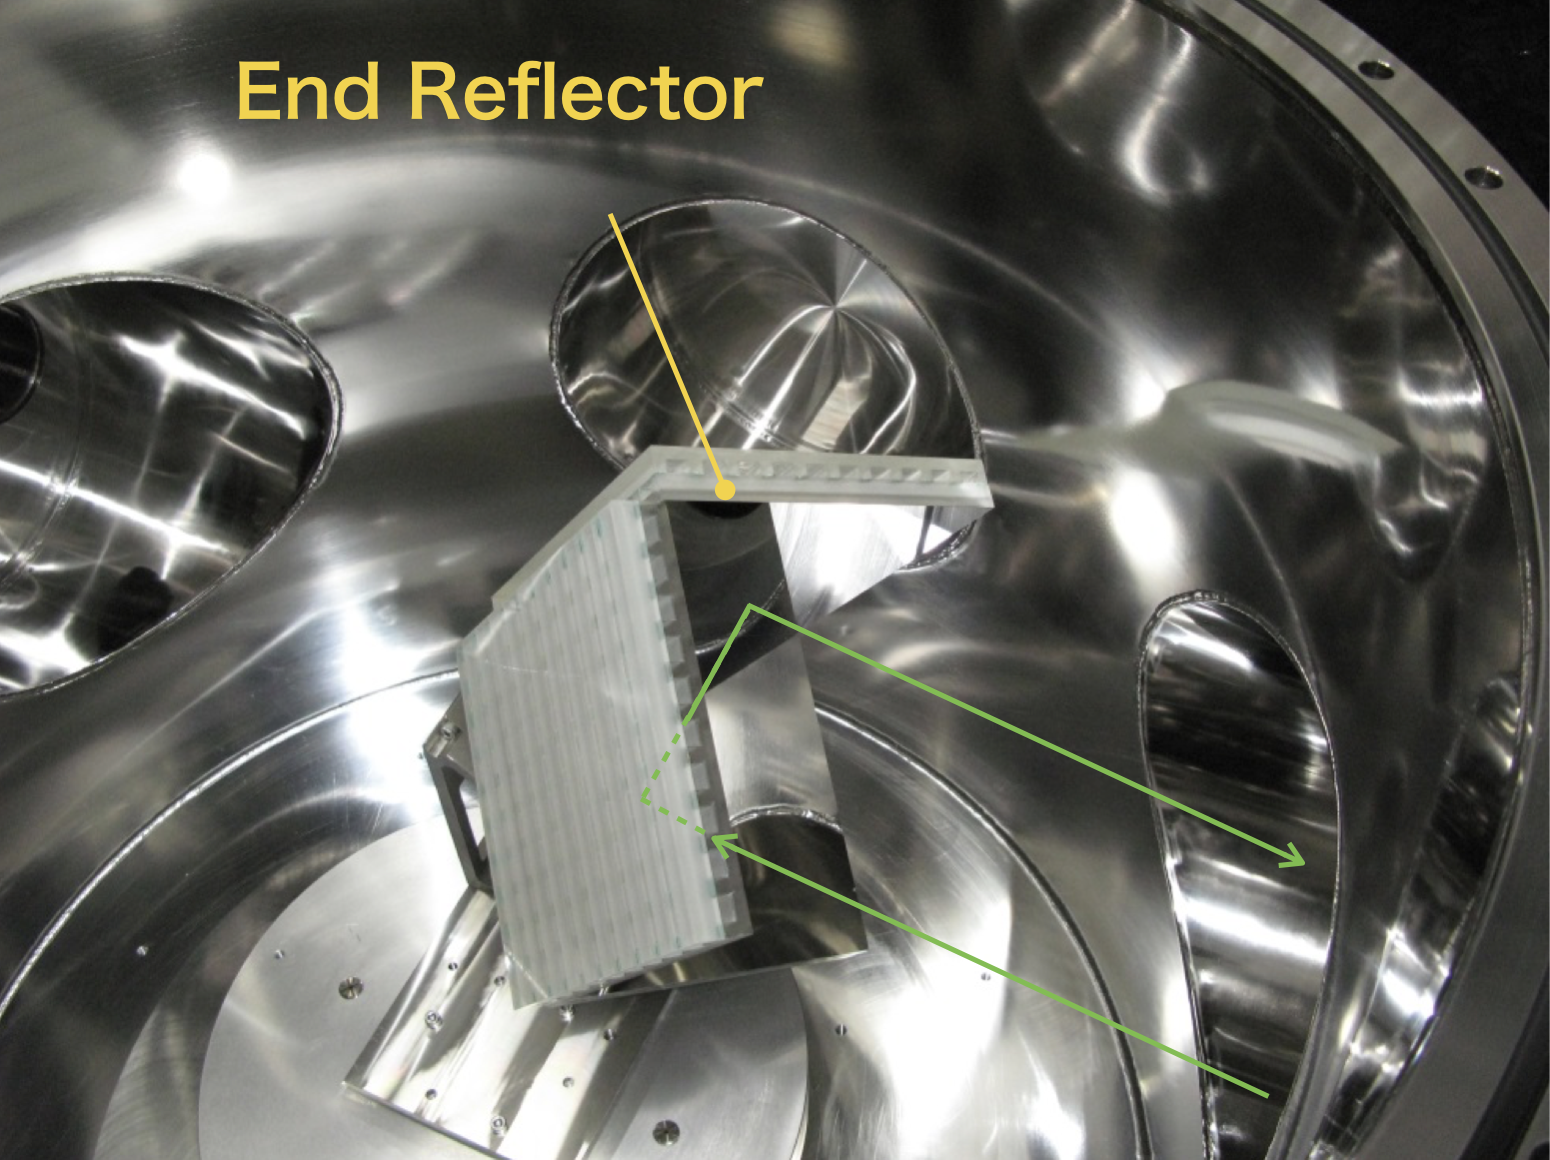
\includegraphics[width=11cm]{./img_chap4/img419.png } %ファイル重い
      
\includegraphics[width=11cm]{./img.png}      
      \subcaption{Core optics in the end vacuum chamber. }\label{img:img419}
    \end{center}
    \caption{..}
\end{figure}


\subsection{Frequency Stabilized Laser}

周波数安定を行っている。

\begin{figure}[h]
  \begin{center}   
    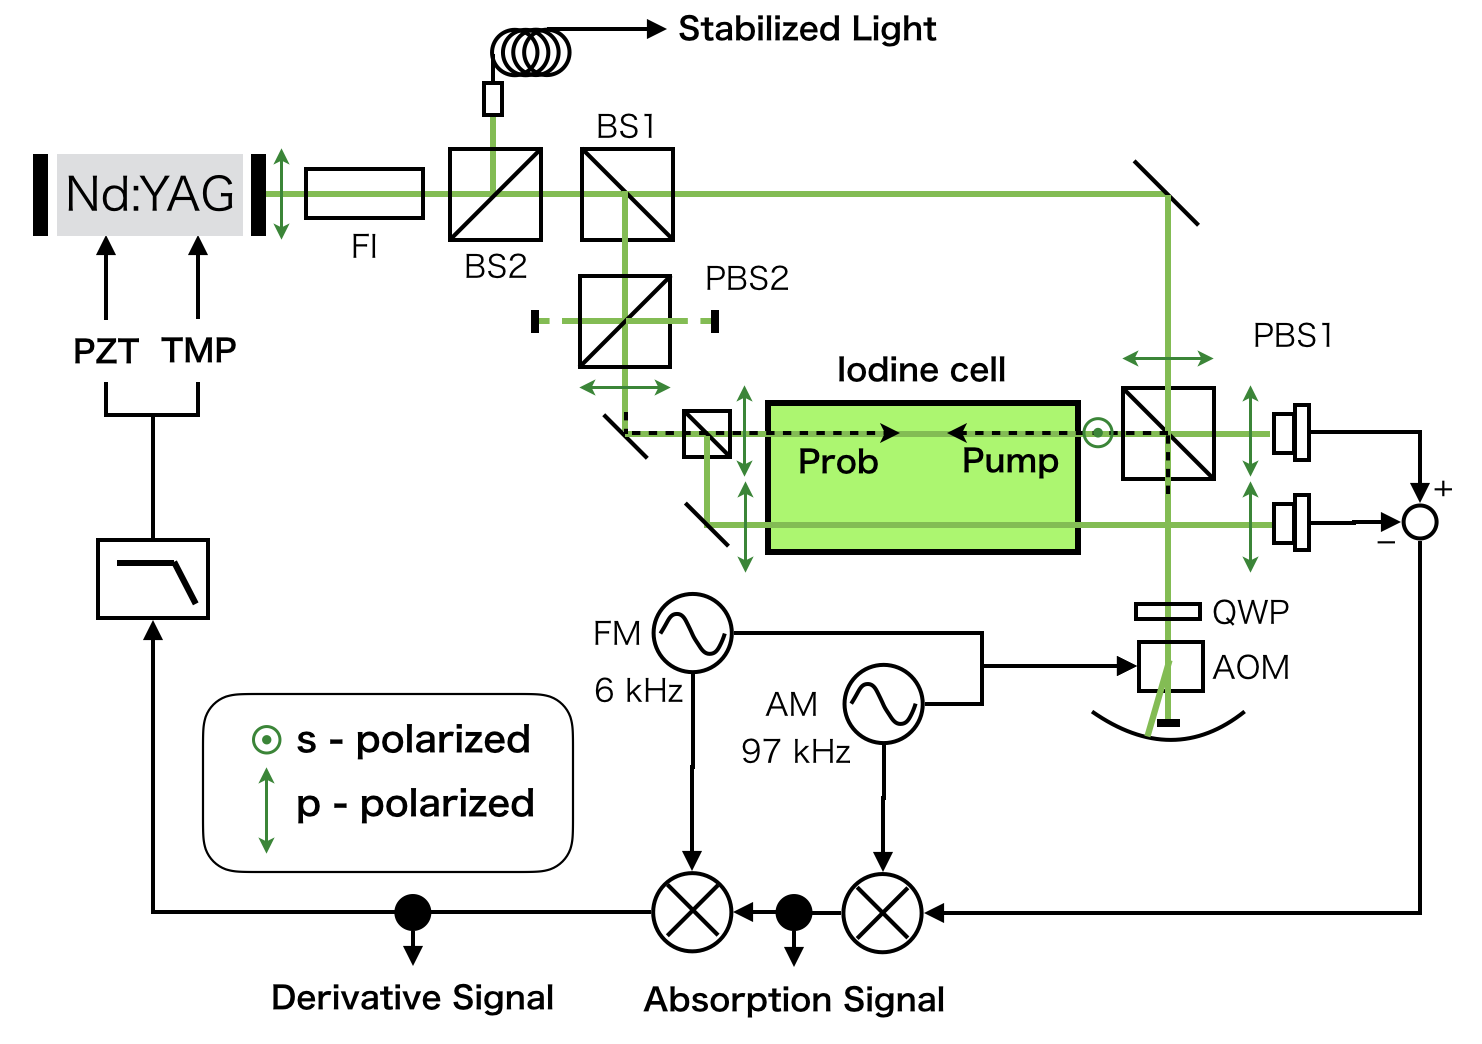
\includegraphics[width=11cm]{./img_chap4/img417.png}
    \caption{Schematic diagram of the frequency-stabilization system of the GIF main laser.}\label{img:img417}
  \end{center}
\end{figure}

\section{Data Aquisition System}
\subsection{Realtime Processing}


\subsection{...}



\section{Summary of the Chapter} %章のまとめ
本章で述べたパラメータを表にまとめる。
